\chapter{Results}

\emph{\color{gray}Probably add astigmatism correction observation results to Experimental when optical flat is talked about.}

\emph{\color{gray}Also in Experimental -- probably need to mention CCD digitaztion pedestal and noise, and dark counts which are zero when cold.  ALSO:  add (C480) after mention of Coumarin 480 (in Experimental).}

\textbf{\color{red}Where did you say to write how defocused alignment is done (i.e., find focus, then defocus and center fluorescence)?  I think it should be said before discussion (or w/) of excit spec since it's used there (as well as for bleaching).}

Studies of several emission peaks of neutral Ba in SXe are discussed in \ref{sec:fluorescence}.  Temperature and annealing dependence are discussed in \ref{subsec:tempanneal}, and bleaching of these peaks is discussed in detail in \ref{subsec:bleaching}.  Imaging of Ba fluorescence in a focused laser region is discussed in \ref{imaging}, with the ultimate achievement of imaging at the single atom level using the 619-nm fluorescence peak.  Candidate fluorescence peaks of Ba\textsuperscript{+} in SXe are reported in \ref{sec:BaPlus}.

\section{Fluorescence of Ba in SXe}
\label{sec:fluorescence}

Deposits of Ba in SXe absorb primarily between 540~nm and 570~nm.  An absorption spectrum, obtained by observing absorption of white light by a large Ba deposit at 11~K, is shown in Fig. \ref{fig:BaAbs}, along with an example emission spectrum with excitation at 557~nm.  Significant broadening, as well as a 4-nm redshift  of the central peak, occur relative to the vacuum $6s^{2}$ $^{1}$S$_{0} \rightarrow 6s6p$ $^{1}$P$_{1}$ absorption value of 553.5~nm.  Initial discovery of this absorption and emission was done with the purely neutral Ba getter source.  Observation of the same spectra from Ba\textsuperscript{+} ion beam deposits demonstrates some neutralization of the ions.  The fraction of ions neutralized is not determined.  \cite{Mong2015,Shon,Brian}

\begin{figure} %[H]
        \centering
                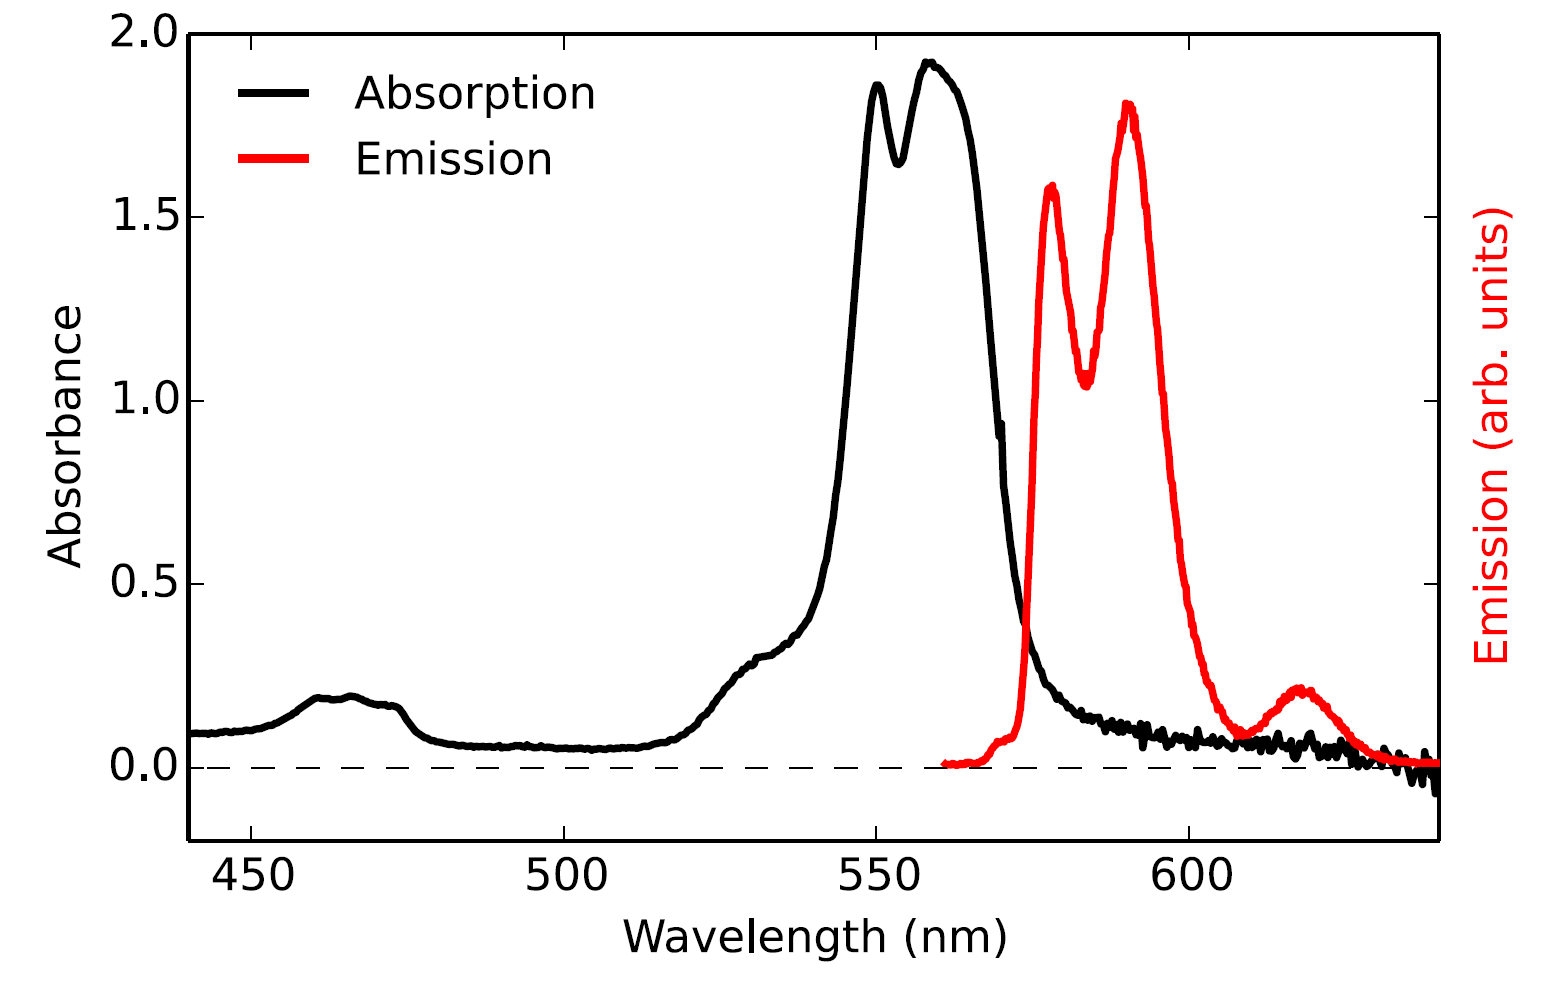
\includegraphics[width=.7\textwidth]{figures/BaAbs_fromBaSpec.png}
                \caption{Absorption and emission spectra of neutral Ba in SXe.  \cite{Mong2015}}
\label{fig:BaAbs}
\end{figure}

\begin{figure} %[H]
        \centering
                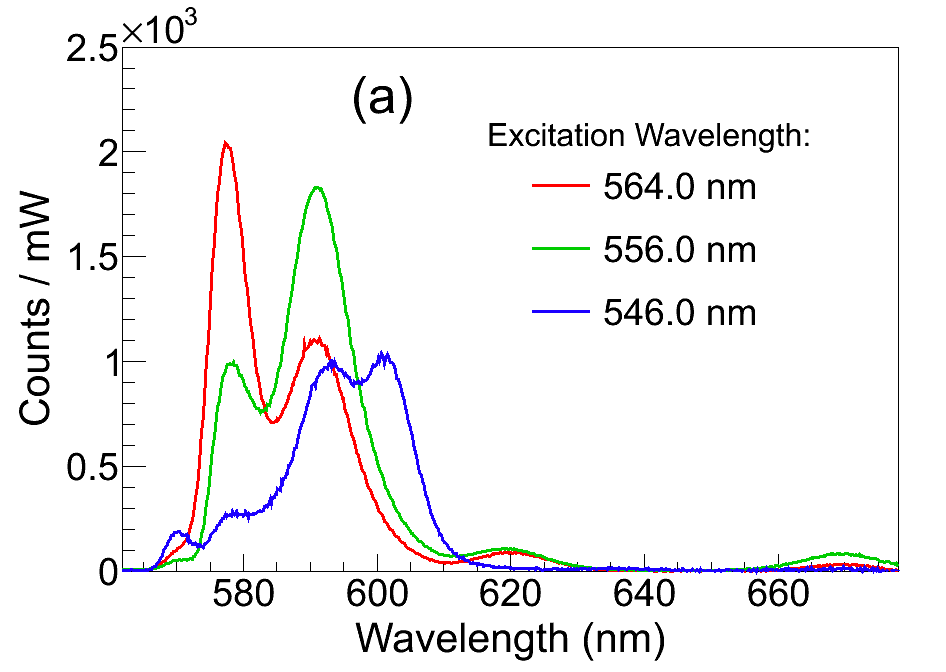
\includegraphics[width=.5\textwidth]{figures/excitspec_grn_spectra_v2.png}
                ~
                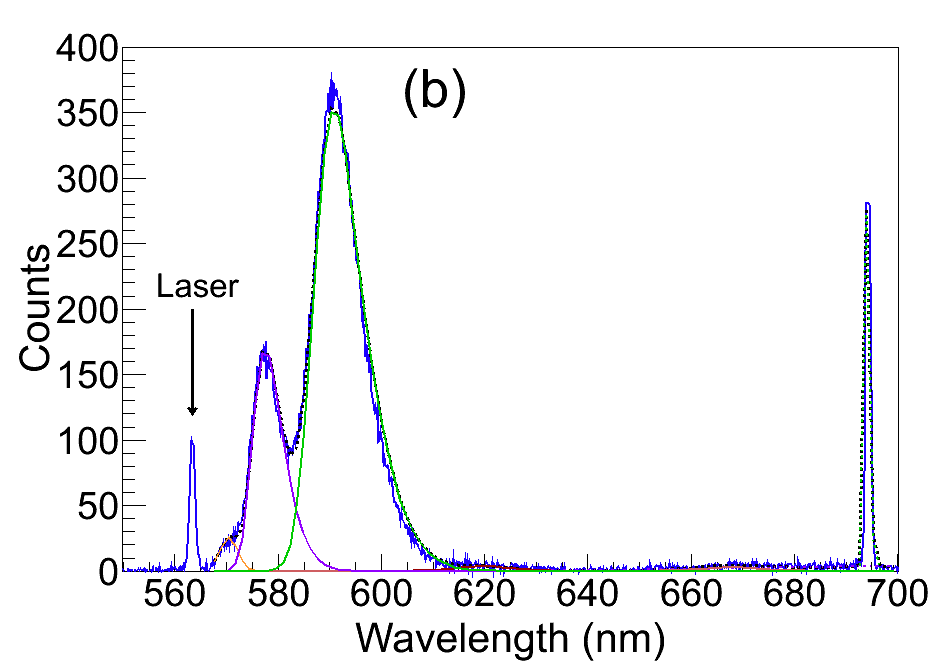
\includegraphics[width=.5\textwidth]{figures/excitspec_grn_spectra_fit.png}
                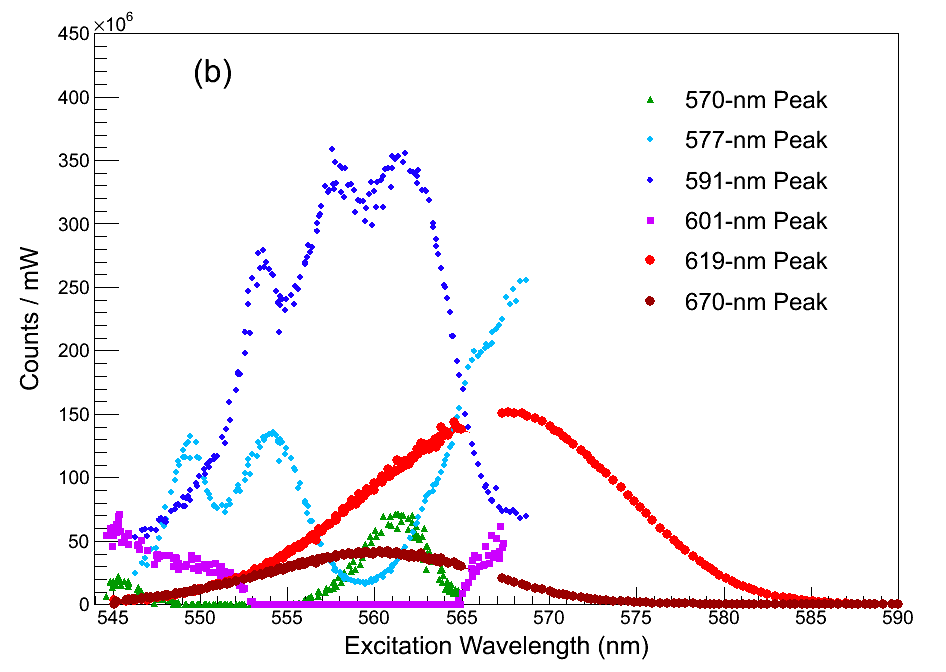
\includegraphics[width=.95\textwidth]{figures/excitspec_grn.png}
                \caption{Background-subtracted fluorescence spectra for a few different excitation wavelengths (a), an example fit to a spectrum (b), and full excitation spectra for all observed Ba fluorescence peaks (c).  Magnitudes in (c) have been scaled for visibility on the same plot (relative magnitudes are arbitrary as they are affected by relative site populations and fluorescence efficiencies).  The discontinuity around 566~nm for the 619- and 670-nm peaks is the boundary between usage of different laser dyes.  R6G dye is used for higher wavelengths and R110 for lower wavelengths and for all other curves.  Curves for the R6G segments (619- and 670-nm peaks) require special scaling to line up with their respective R110 segments, and this scaling was different between the 619- and 670-nm peaks, likely due to different relative populations of those sites on the different deposits.}
\label{fig:excitspecGrn}
\end{figure}

%\begin{equation}
%A(1+erf(\frac{x-a}{\sigma_{1}})(1-erf(\frac{x-a}{\sigma_{2}}))
%\label{eqn:specfit}
%\end{equation}

The several red-shifted emission peaks observed are attributed to Ba atoms occupying different matrix sites in the SXe.  Deposition at temperatures higher than 11~K and exploration of more excitation wavelengths have led to discovery of a few emission peaks beyond the 591- and 577-nm peaks reported in \cite{Shon} and \cite{Brian}.  Emission spectra for selected excitation wavelengths are shown in Fig. \ref{fig:excitspecGrn}(a), for a deposit made at 44~K and observed at 11~K.  These selections are part of a full excitation spectrum, shown in Fig. \ref{fig:excitspecGrn}(c).  An excitation spectrum is produced by scanning the dye laser and measuring the magnitude of each fluorescence peak vs. excitation wavelength.  For each 1-s CCD exposure, a sum of asymmetric Gaussian functions is fit to the spectrum after pedestal subtraction.  The fit function used is $A(1+$erf$(\frac{x-a}{\sigma_{1}})(1-$erf$(\frac{x-a}{\sigma_{2}}))$, where $A$ is the free amplitude parameter.  The peak position $a$ is fixed for each peak, as are the left and right smearing widths $\sigma_{1}$ and $\sigma_{2}$.  The function erf() is a Gaussian error function.  This asymmetric Gaussian function works better than a standard Gaussian or Lorentzian, but still is not perfect for all frames, as the shape of the emission can depend on the excitation wavelength.  An example frame with fits is shown in Fig. \ref{fig:excitspecGrn}(b).  The full fit is the dotted black line, and each peak's contribution is in color.  Curves in (a) have about 100$\times$ the laser power used in the excitation spectrum (e.g. (b)) where low intensity is desired to avoid bleaching during the scan.  Rather than attempting frame-by-frame background subtractions, additional Gaussians are fit to the broad and sharp background fluorescence.  These backgrounds and their excitation spectra are discussed in \ref{sec:bgs}.  A 566~nm Raman filter is used to attenuate the majority of the laser scatter, however the small amount of scatter passed by the filter is used to determine the frame's excitation wavelength.  Each peak's fit contribution is then integrated and scaled by the frame's laser power, as the power output is not constant through the dye range.

%\emph{\color{gray}Care about 10~K excitation spectrum?}

Wavelength calibration is done using three lasers whose wavelengths are first measured with a Burleigh Wavemeter:  a red diode laser at 656.99~nm, a doubled Nd:YAG laser at 532.23~nm, and the C480 blue dye laser typically around 475~nm (at 488.91~nm for the data in Fig. \ref{fig:excitspecGrn}).  These lasers were directed at the same position on the sapphire window, and their scatter is imaged along the same path as the Ba fluorescence.  The WinSpec software applies the diffraction grating equation to calibrate each CCD pixel to a wavelength.

\subsection{Annealing/Temperature Dependence}
\label{subsec:tempanneal}

%\emph{\color{gray}When does it need to be mentioned that certain data was also used in the paper(s)?}

Matrix site occupancies for Ba atoms can depend on annealing history, and similarly on the temperature at which a deposit is made.  Spectra under different temperature conditions are shown in Fig. \ref{fig:specTempConditions}.  Peak shapes look similar for deposits made at 40-55~K as those made at 11~K and then annealed to 40-55~K, both being observed at 11~K, though relative amplitudes are not the same, likely due to matrix site populations.  Without annealing, 11-K deposits have a different peak shape around 590~nm, with a broader peak centered around 596~nm.  Another possibility is that the broader shape is due to a higher population of the 601-nm peak, and it is not resolved from the 591-nm peak.

\begin{figure} %[H]
        \centering
                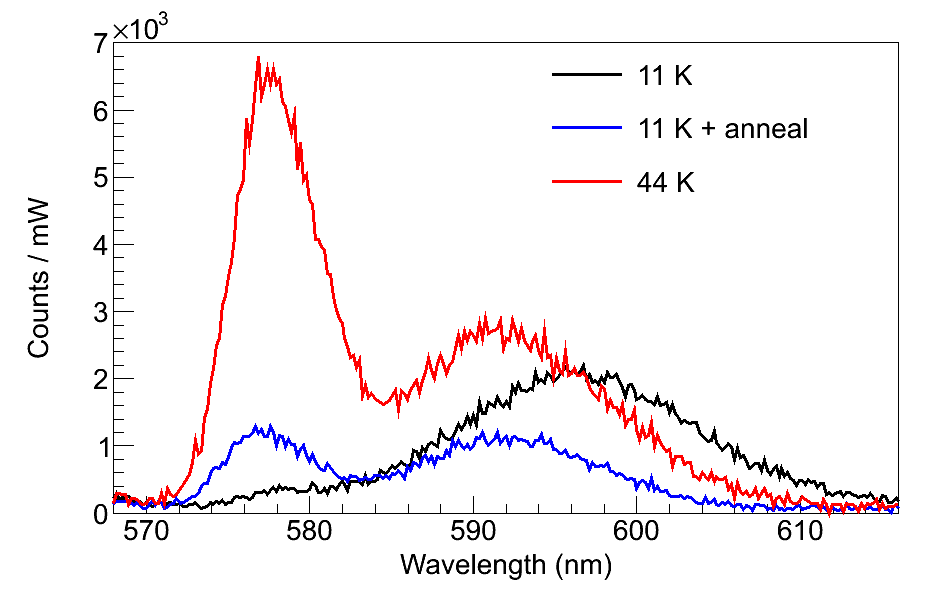
\includegraphics[width=.7\textwidth]{figures/spectra_temperature_conditions.png}
                \caption{Spectra of peaks around 590~nm of a Ba\textsuperscript{+} deposit made at 11~K before and after annealing to 39.4~K, and one made at 44~K.  All observations are at 11~K.  Both Ba\textsuperscript{+} deposits are 15~s, however the 44~K deposit is scaled slightly to account for different ion current.  Laser power was about 0.1~mW with an unfocused beam waist of w = 7.056~mm, at 566~nm wavelength.}
\label{fig:specTempConditions}
\end{figure}

Fluorescence spectra with 564~nm excitation through several annealing cycles for a deposit made at 11~K are shown in Fig. \ref{fig:specAnneal}.  At this wavelength, all observed Ba peaks are prominent except the 570-nm peak.  Similar to excitation spectra, individual fluorescence peak amplitudes can be plotted vs. temperature by fitting the full spectrum in each frame.  Rather than asymmetric Gaussians, this analysis used standard Gaussian and Lorentzian functions.  Lorentzians fit the 619-nm and 670-nm peaks well.  Each individual peak's amplitude is plotted vs. temperature in Fig. \ref{fig:annealGrn}(b-f), with an example of a fit spectrum in Fig. \ref{fig:annealGrn}(a).  In this interpretation, the 601-nm \emph{\textbf{\color{red}Is it similar to the 601 fit in excit spec?}} peak along with the 591-nm peak fit the broader peak in the initial 11~K deposit.  The 601-nm peak shows nearly complete loss in the first anneal cycle.  The 670-nm peak sees significant loss, with more loss with each succeeding anneal cycle, each of which reach higher temperatures.  The 591-nm sees moderate loss with each cycle.  The 577-nm and 619-nm peaks gain significantly with the first anneal \emph{\color{gray}refer to 50~K vs 11~K deposit plot showing higher 619 here, or is that somewhere else now, like near spectra condistions plot?}, suggesting that they are due to more stable matrix sites.  Both peaks remain about the same after the second cycle (small gain in 577-nm), and both see loss after the third cycle, which reaches the higher temperature of 48~K. \emph{\color{gray}Either just say this could be due to diffusion (or something else?), or was there a specific temperature to reference from that paper?}

\emph{\color{gray}A conclusion is that we deposit at around 50~K ($\pm 5$) in experiments for more signal in 619 as well as 591/577.}

\begin{figure} %[H]
        \centering
                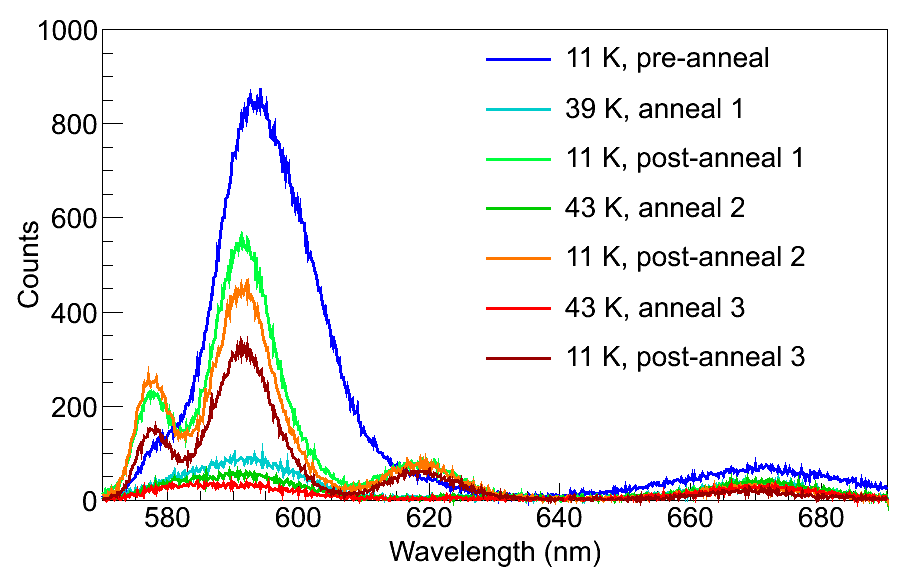
\includegraphics[width=.95\textwidth]{figures/spectra_annealing.png}
                \caption{Spectra of a large Ba\textsuperscript{+} deposit through several annealing cycles.  Initial deposit was at 11~K.  Laser power was about 0.2~mW with an unfocused beam waist of w = 7.056~mm, at 564~nm wavelength.  \emph{\color{red}This same data, but a different plot, is in BaSpec, as is some of the annealing plots -- do I just cite the paper or what?}}
\label{fig:specAnneal}
\end{figure}

\begin{figure} %[H]
        \centering
                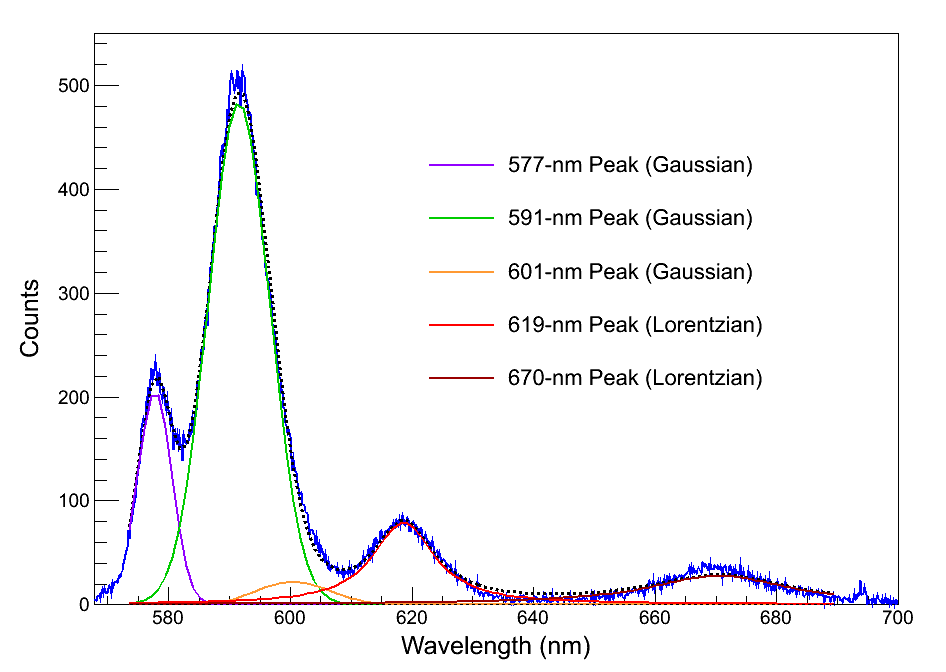
\includegraphics[width=.5\textwidth]{figures/spectra_anneal_fit.png}
                ~
                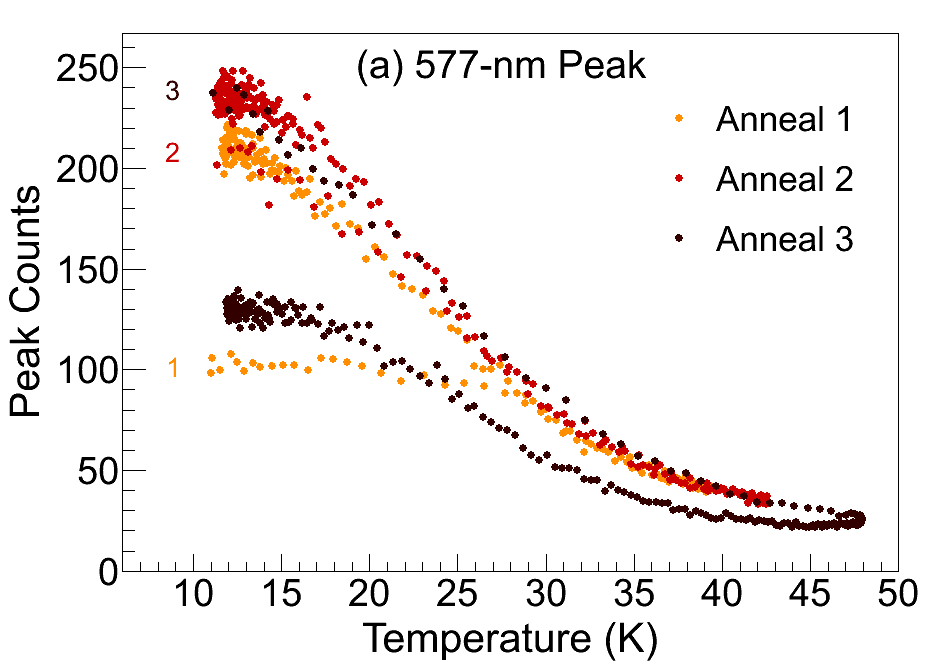
\includegraphics[width=.5\textwidth]{figures/anneal_577peak.png}
                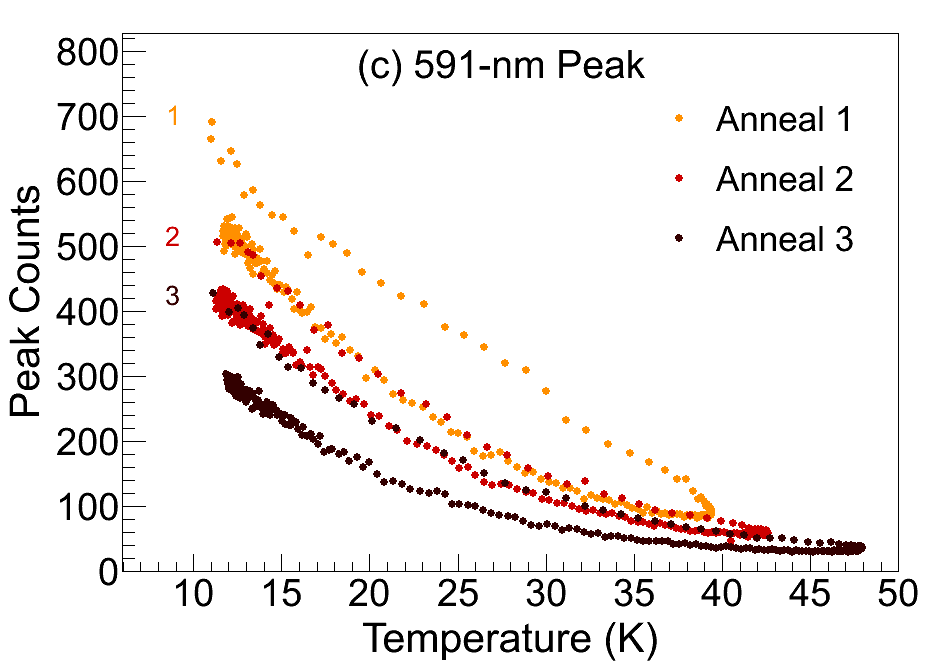
\includegraphics[width=.5\textwidth]{figures/anneal_591peak.png}
                ~
                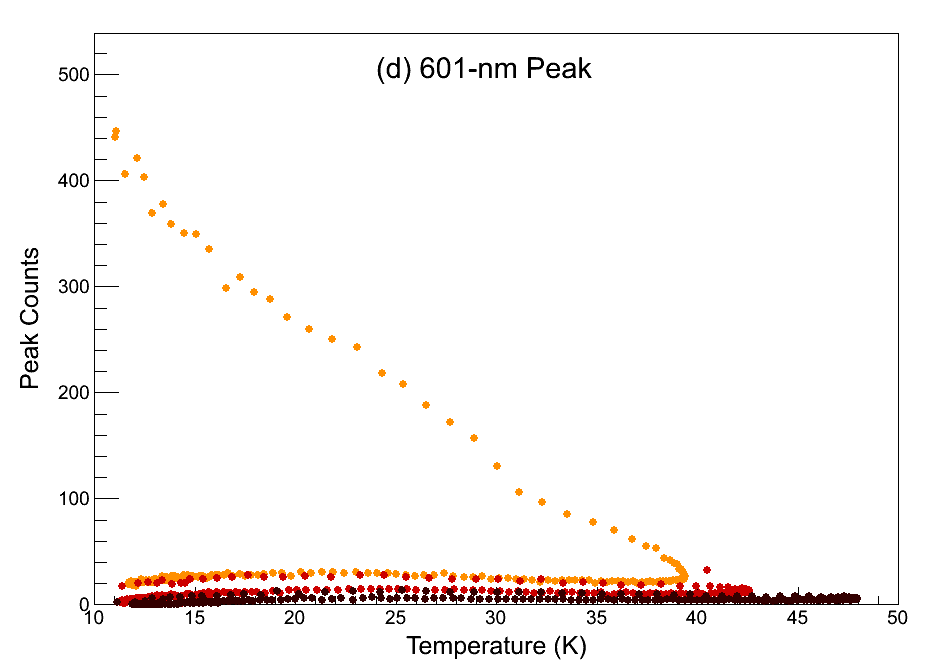
\includegraphics[width=.5\textwidth]{figures/anneal_601peak.png}
                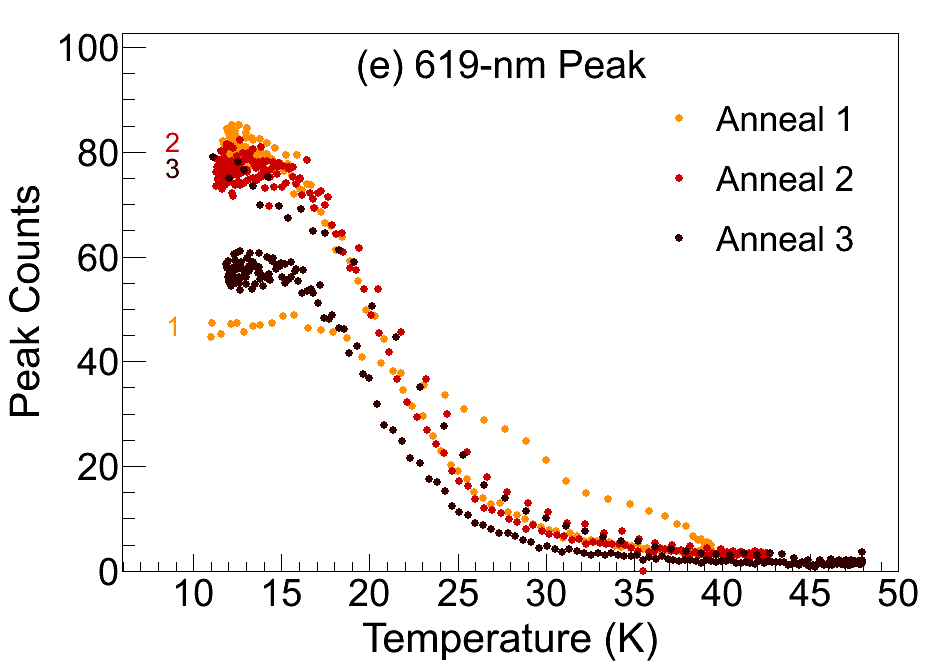
\includegraphics[width=.5\textwidth]{figures/anneal_619peak.png}
                ~
                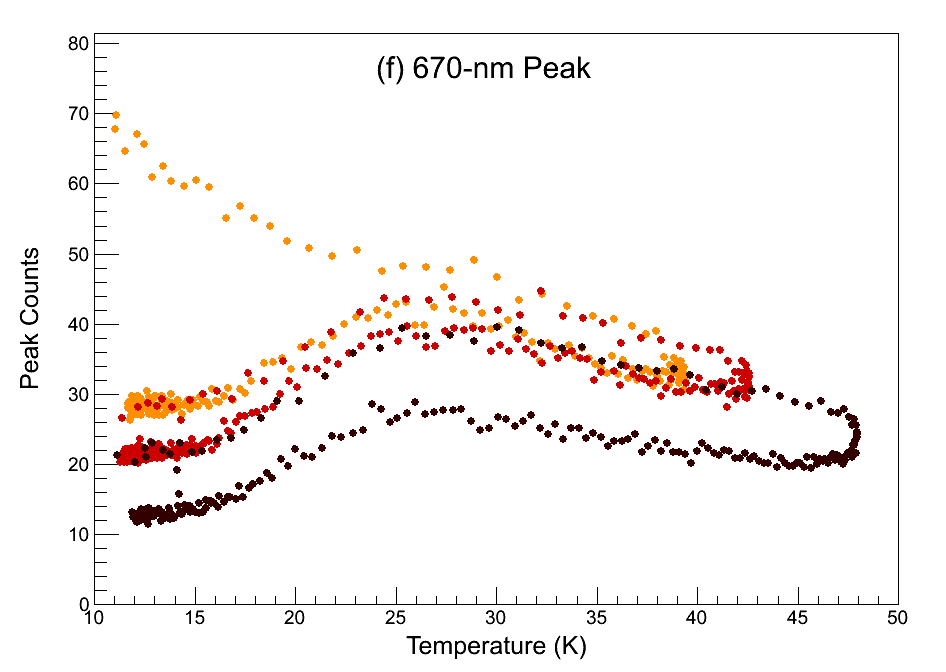
\includegraphics[width=.5\textwidth]{figures/anneal_670peak.png}
                \caption{\color{red}Needs legends for anneals -- just on one?  Needs larger text, and thicker border? Prolly test that on excitspec to coincide with larger plot.  (a) needs (a).  Want 1 2 3 on anneals?}
\label{fig:annealGrn}
\end{figure}

Aside from matrix site changes, direct temperature dependence of fluorescence is observed in annealing cycles.  The 577-, 591- and 619-nm peaks have their highest amplitude at 11~K.  The 577-nm and 619-nm peaks appear to be leveled off at 11~K, while the 591-nm may benefit from even lower temperatures.  The 670-nm peak has its highest amplitude at around 25~K (apparent after its major site alteration has occurred).  \emph{\color{gray}601 and (not shown) 570 would require different wavelength to study.} \emph{\color{gray}This [loss of flu at higher temp] suggests that a probe in nEXO will need to be moved to an evacuated chamber in order to cool to 11~K or below for observation.}

%[inverse relationship] could be due to a different matrix environment at higher temperature, or possibly a loss of fluorescence efficiency due to increased non-radiative decays from the excited state.  

\subsection{Bleaching}
\label{subsec:bleaching}

\emph{\color{gray}Describe how you align here -- observe focused image, find its focus, and defocus by an amount, then centering the broad Ba fluorescence for a known intensity region of x\% ... \textbf{do you want an explanation of the image in experimental?  or maybe this is a good place to introduce it?}}

({\color{red}do a correction on p-meter sensitive area and on p-meter quantum efficiency, and also a spherical aberation correction for power, though that may not matter for the defocused studies.})

590 etc, model fit (see results intro paragraph)

\begin{figure} %[H]
        \centering
                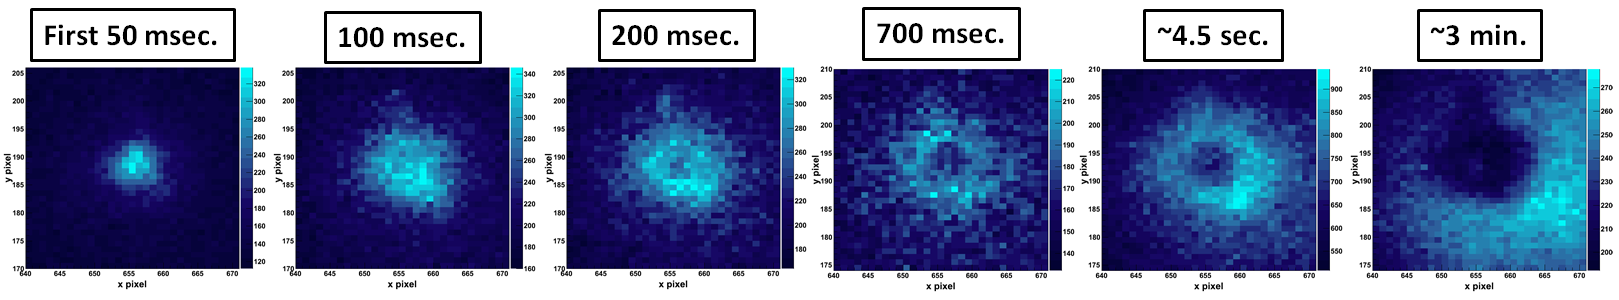
\includegraphics[width=.9\textwidth]{figures/hole_bleach_590.png}
                \caption{}
\label{fig:testfig}
\end{figure}

Repump attempts -- nothing found with cheap lasers.

619, with the changes in time and I

bleaching effect on excit spec (bleaching site change search)

\section{Backgrounds}
\label{sec:bgs}

One source of background in spectra and images is fluorescence from the sapphire window.  A spectrum of this fluorescence with x~nm excitation is shown in Fig. [fig sapphire spectrum](a).  The strong, sharp peak at \emph{\color{gray}(peaks around? May need to ask Bill about what peaks exist and at what temps)} x~nm are a well-known fluorescence of Cr\textsuperscript{3+} impurities in the sapphire bulk.  \emph{\color{gray}Is only one of the lines (the one mentioned on wikipedia) strong at room temp?  I think you have room temp soectra somewhere.}  A weaker and much broader fluorescence is observed, also from the sapphire bulk, which reaches into the wavelength regions of the Ba fluorescence peaks.  The excitation spectra for these fluorescence components are shown in Fig. [fig Cr](b), over the range of both R6G and R110 dyes, as well as the blue dye C480.  The excitation spectrum for the {\color{red}693(s?)} Cr\textsuperscript{3+} peak{\color{red}(s)} agrees with the literature [cite that one paper].  The identical excitation spectrum of the broad fluorescence, including the small peaks around x~nm, demonstrate that it too is due to Cr\textsuperscript{3+} in the sapphire.  \emph{\color{gray}\textbf{check this -- was it certainly from just the bulk and not from partly surface BG for those excit. spec.? -- ACTUALLY is it possible that some of this is the surface BG?  Yes, if it was a broad laser, unless the sapphire is really high in these, which maybe it is?}.}  Commercially available c-plane quality sapphire windows contain very low concentrations of Cr\textsuperscript{3+}.  The highest purity windows we have found are from Meller Optics, with Cr\textsuperscript{3+} concentrations of around {\color{red}10 ppt} estimated from our spectra.

Another background emission is observed from the surfaces of the window.  Its broad fluorescence is shown in Fig. [fig 1st order surface BG] with a 610-nm Raman filter cutoff and {\color{red}570~nm} excitation, in a 1\textsuperscript{st}-order image, where the x-axis is wavelength and the y-axis is y position in the image.  The nature of this emission has not been determined, however a few features have been identified.  One is that the emission increases as the window temperature is decreased, down to about 100~K where it is flat down to 11~K, shown in Fig. [fig BG temp dep] along with the temperature dependence of the Cr\textsuperscript{3+} emission, which has the inverse relationship.  Another feature of the surface background is that it bleaches with laser exposure, shown in Fig. [fig surfaceBG bleaching].  This useful in that the background can be reduced by pre-bleaching of the window.  However, the bleaching behavior also presents a nuisance.  Frequent Xe-only deposits must be made in order to establish proper background subtraction, as historical bleaching and possible slight movements of the laser to differently bleached positions can cause variation in the background over en experiment period.  Spacial variation in the background is especially cumbersome in a laser scanning experiment, as discussed in xxx.  Given these behaviors, it is possible that the surface background is caused by a species which freezes to the window, or something which coats the window and fluoresces more at lower temperatures.  In either case, the bleaching could be explained by evaporation with laser heating, or by optical pumping of the species into a metastable state.

\section{Imaging}
\label{imaging}

Though the imaging spectrometer can produce spacial images with the 0-order grating reflection, better collection efficiency and imaging quality are achieved by removing the spectrometer and imaging directly onto the CCD.  Band-pass filters are used to pass the desired Ba fluorescence peak(s) while attenuating laser scatter and sapphire fluorescence.

An example image of the focused 570~nm dye laser passing through a c-plane sapphire window of thickness 0.5~mm, using the 620-nm band-pass filter on the fluorescence, is shown in Fig. [fig example image].  With 4$\times$ magnification, each pixel is 5~$\mu$m $\times$ 5~$\mu$m.  The laser's path through the window is faintly visible by the tail of the broad Cr\textsuperscript{3+} fluorescence in the 620-nm region (see Fig. [fig band passes on spectrum with BG and Ba fluorescence shown] for regions passes by various filters).  The laser is focused at the top surface of the window, which faces the ion beam.  The surface background is seen on both surfaces.  The observed size of the laser spot, with a 1/e$^{2}$ radius of about 12~$\mu$m, is larger than the 2.06~$\mu$m $\times$ 2.66~$\mu$m 1/e$^{2}$ laser spot size.  Aberrations and vibrations in the collection optics could contribute to this inability to reach the diffraction limit in imaging.

\subsection{Vibrations and Effective Laser Region}

Relative vibrations between the laser and sapphire window will affect the number of Ba atoms exposed, increasing the effective laser spot size.  This was studied by observing the position of a ``dust spot" (a highly scattering feature on the sapphire window) relative to the position of the laser in an image on time scales down to 50~ms.  An example of an image from this experiment is shown in Fig. [fig dust spot vibe image].  The 570-nm dye laser is somewhat de-focused, and the dust spot is illuminated by a de-focused {\color{red}657~nm} diode laser. For each frame, 2D Gaussian functions are fit to locate the center of the laser spot and the dust spot in order to measure their relative position.  The fit for the laser spot is restricted in y so that it is not affected by the bulk sapphire fluorescence path.  The difference between dust spot and laser positions is plotted in Fig. [fig vibe vs. time with sine fit] for both x and y.  Each exposure in this plot is 50~ms, though readout time and camera shutter compensation time result in x~s between frames.  The best fit of a sine function results in a vibration frequency of x~Hz.  This is consistent with the audible frequency of the cryostat He pump.

To calculate an effective laser spot size due to this vibration, each difference (x,y) between laser and dust spot is used as the center of a 2D Gaussian, each with w$_{x} = 2.06~\mu$m and w$_{y} = 2.66~\mu$m to represent the laser spot.  Such Gaussian functions are summed to all points to produce a distribution of summed laser exposure, shown in Fig. [fig vibe sum 2D].  The total area enclosed by a 1/e contour then represents the effective area.  Since x and y movement is correlated, and since the movement is sinusoidal, the effective area is only about 2$\times$ the real laser spot size, and the effective laser region is {\color{red}17.6}~$\mu$m$^{2}$.

The aforementioned is the most concerning vibration to understand.  Vibration of the laser itself is included in that study.  Vibration of the collection optics will affect the imaging resolution, but not the number of atoms being observed.  These vibrations are minimized by stable mounts.

\subsection{Imaging 577- and 591-nm peaks}

First attempts at imaging small numbers of Ba atoms in a focused laser region were done with the 577- and 591-nm Ba fluorescence peaks together using a {\color{red}579-nm} band-pass filter (Fig. [fig band passes on spectrum with BG and Ba fluorescence shown]).  This filter has a 2" diameter, resulting in a factor of 4$\times$ more collection efficiency.  Bleaching data is used to optimize laser intensity and exposure time to achieve maximal signal in frame 1, and to avoid hole bleaching.  The fast bleaching of these peaks is the limiting factor on sensitivity.  An image of $\leq$ 10$^{4}$ atoms (10$^{4}$ Ba\textsuperscript{+} ions deposited into the effective laser region) is shown in Fig. [fig 590-lines image].  At only x total counts, this is near the limit of sensitivity.  As discussed in xxx, detection of very small numbers of atoms in these sites may require several infrared re-pump lasers.  As a result of low total exposure, neither the sapphire nor the surface backgrounds are present in these images.

\subsection{Imaging 619-nm peak}

um

\begin{figure} %[H]
        \centering
                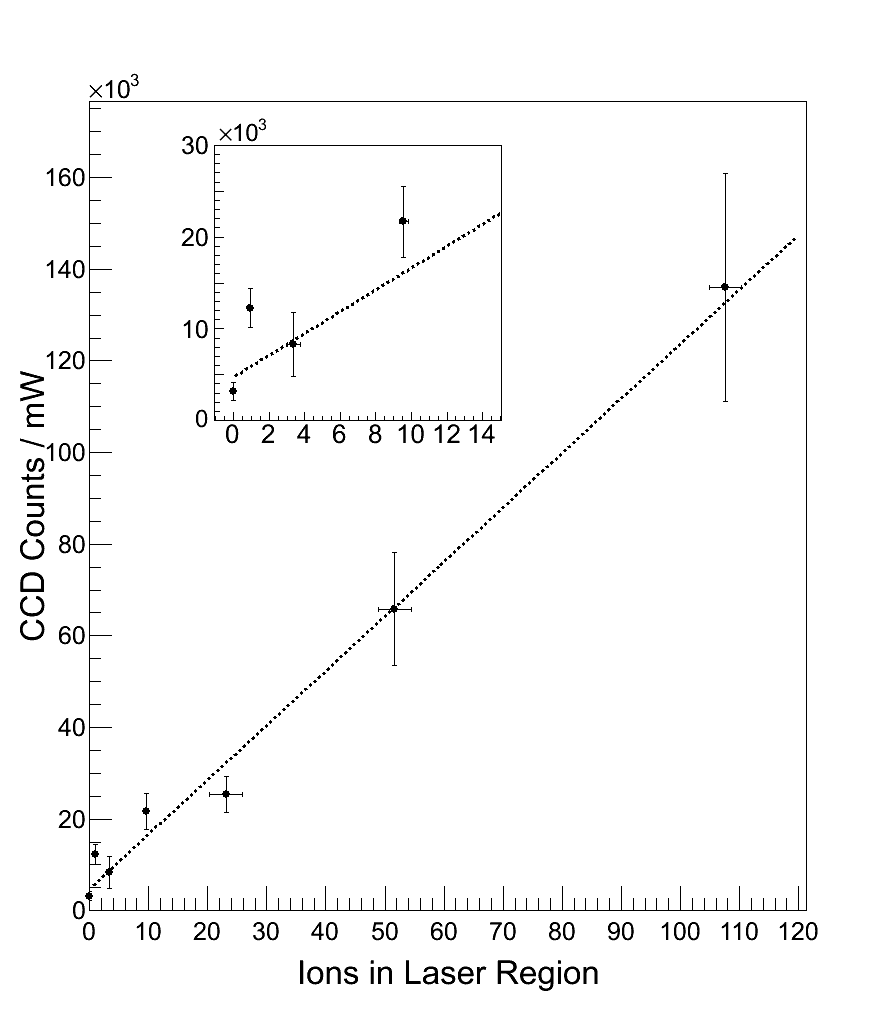
\includegraphics[width=.7\textwidth]{figures/fitgrouped_20150807_20150916_inset.png}
                \caption{Combined 2015-08-07 and 2015-09-16 with statistical errors.  \emph{\color{gray}Move y-axis title over.}}
\label{fig:lin}
\end{figure}

\subsection{Further Checks on 619-nm Peak}
\label{subsec:619identification}

The 619-nm peak, as well as the 670-nm peak, is attributed to neutral Ba by a few further tests.  A large Ba\textsuperscript{+} deposit is compared to a deposit made with the Ba getter in Fig. [fig Ba+/Ba/Ar+].  The 619-nm and 670-nm peaks are observed with both sources, and since the getter produces only neutral Ba, they are attributed to neutralized ions in Ba\textsuperscript{+} deposits.  Observation of the fluorescence with two different types of Ba sources is itself positive.  In addition, observation of the fluorescence with the low deposit energy of the getter may bode well for the prospect of grabbing on a probe in LXe.  Observation of a large deposit of Ar\textsuperscript{+} in SXe is also shown in Fig. [].  The lack of fluorescence further rules out a matrix-damage-related source of the fluorescence, such as color centers.  \emph{\color{gray}Ar+ pulsing lack of flu.}.

\emph{\color{gray}Whatever you did with the extra-filter-pass check (IR etc.)}

\emph{\color{gray}Also have stuff on ruling out extra-BP stuff, and something else I think.}

Leak rate dependence -- ``Leak rates resulting in [x nm/s $\rightarrow$ 1:xxx Ba:Xe] optimize fluorescence, which is consistent with rates where Ba-Ba interactions are minimized [ref?] \emph{\color{gray}(are there other explanation?  check the gas oxidation thing.)}.  Rates higher than this result in rapid frosting ..." \emph{\textbf{\color{gray}May also just put this at the end of the  Fluorescence section.}}

\section{Candidate Ba\textsuperscript{+} Lines}
\label{sec:BaPlus}

Mention 520~nm peak.